%!TEX root = ../template.tex
%%%%%%%%%%%%%%%%%%%%%%%%%%%%%%%%%%%%%%%%%%%%%%%%%%%%%%%%%%%%%%%%%%%%
%% chapter4.tex
%% NOVA thesis document file
%%
%% Chapter with lots of dummy text
%%%%%%%%%%%%%%%%%%%%%%%%%%%%%%%%%%%%%%%%%%%%%%%%%%%%%%%%%%%%%%%%%%%%

\typeout{NT FILE chapter4.tex}%

\chapter{Implementation}
\label{cha:implementation}

\paragraph{}In this chapter, the implementation of the different modules 
and components mentioned in the previous chapter will be described, 
as well as their process of creation and integration into the 
full system.

\section{Software}
\label{sec:software}
\paragraph{}Since this system is composed of several different components that need 
to run independantly, the software used will need to be robust enough to account for 
each component's requirements, and for this task there the \gls{ROS} framework is used.
There are two versions of this framework, \gls{ROS} and \gls{ROS2}, the latter being the 
most recent version, which is the one to be used in this project.

\subsection{ROS2}
\label{subsec:ros2}
\paragraph{}The \gls{ROS2} framework is a set of software libraries and tools that 
help developers create robotic applications. It is provides a set of solutions to various 
problems, such as parallelism, communication, modularity, and hardware abstraction.

It works by creating a network of nodes (python or c++ programs) that can communicate with each other 
using a publish-subscribe model and a service-client model. The former is a broadcasting 
model where a node can publish messages to a specific topic, and any other 
program can subscribe to that same topic and receive those messages and usse them using callbacks. 
The latter is a request-response model where a specific node is the server and other 
nodes can call it to request a specific service, which helps with modularity 
as each node can have its own specific task and be developed independently. When it comes to 
the hardware abstraction, since the software is wildly used in the robotics community 
it already has a lot of packages and libraries that can be used to interpret data form 
sensors, control actuators, and even simulate the robot in a virtual environment.


\subsection{NAV2}
\label{subsec:navigation2}
\paragraph{}The \gls{NAV2} stack is a set of packages that provide a framework for autonomous navigation. 
It is built on top of \gls{ROS2} and provides a set of tools for coordinating the different components of 
the navigation system.
\begin{figure}[h]
    \centering
    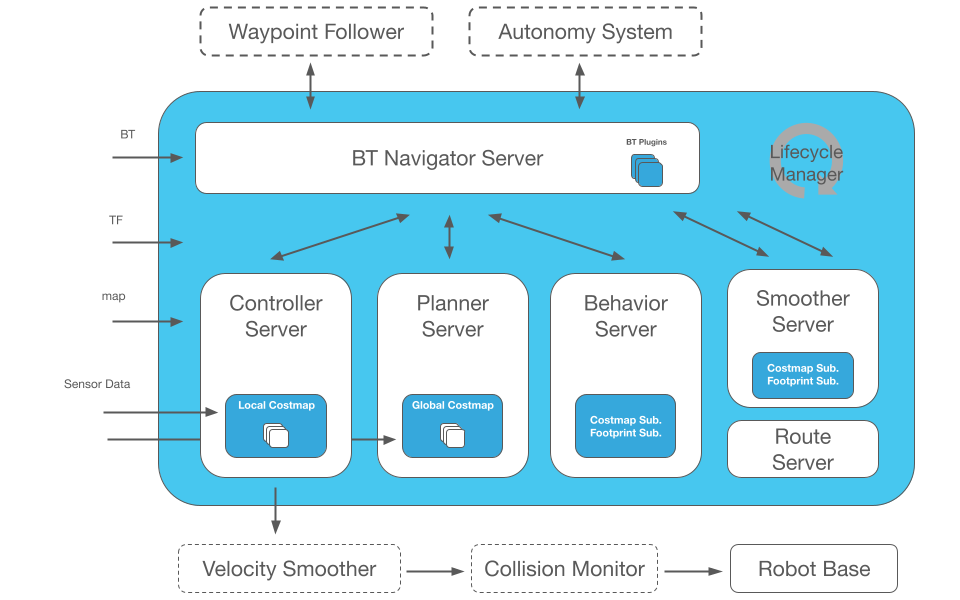
\includegraphics[width=0.8\textwidth]{nav2_architecture.png}
    \caption{NAV2 stack architecture \cite{nav2_architecture}}
    \label{fig:nav2_stack}
\end{figure}

In figure \ref{fig:nav2_stack} we can see the different components of the \gls{NAV2} stack required for 
robust autonomous behaviour. The main components are thr Controller server, which is responsible for, using a controller 
plugin, controlling the robot's movement, the Planner server, which is responsible for, using a custom plugin, 
planning the robot's path, the Behaviour server which, given a custom behaviour tree, is responsible for selecting the 
next action to be taken by the robot, the BT Navigator server, which coordinates all the other servers and the Lifecycle manager 
which controls the lifecycle of the different modules mentioned previously. The stack also includes a variety of already 
defined plugins to be used for localization, path planning and control, however, in this work, a custom planner, controller, 
behaviour tree and also state publisher are created to suit the specific needs of the robot.

\section{Environment}
\label{subsec:environment}
\paragraph{}For development purposes, a virtual environment is used to develop the navigation software 
and test it without the need for a physical robot. This environment can be created using Gazebo, a 
robotics simulator that is compatible with \gls{ROS2}, and it allows the user to create a world in xml format, specifying 
the different physical properties of the environment as well as the structures and objects inside it.

Since the robot will be operating in an agricultural environment, the world created for 
the simulation would have to reflect that, so a simple world was created with five 
corridors with traffic bariers on each side (to simulate trees or crops) and some additional 
obstacles to make for a more complex environment.
\begin{figure}[H]
    \centering
    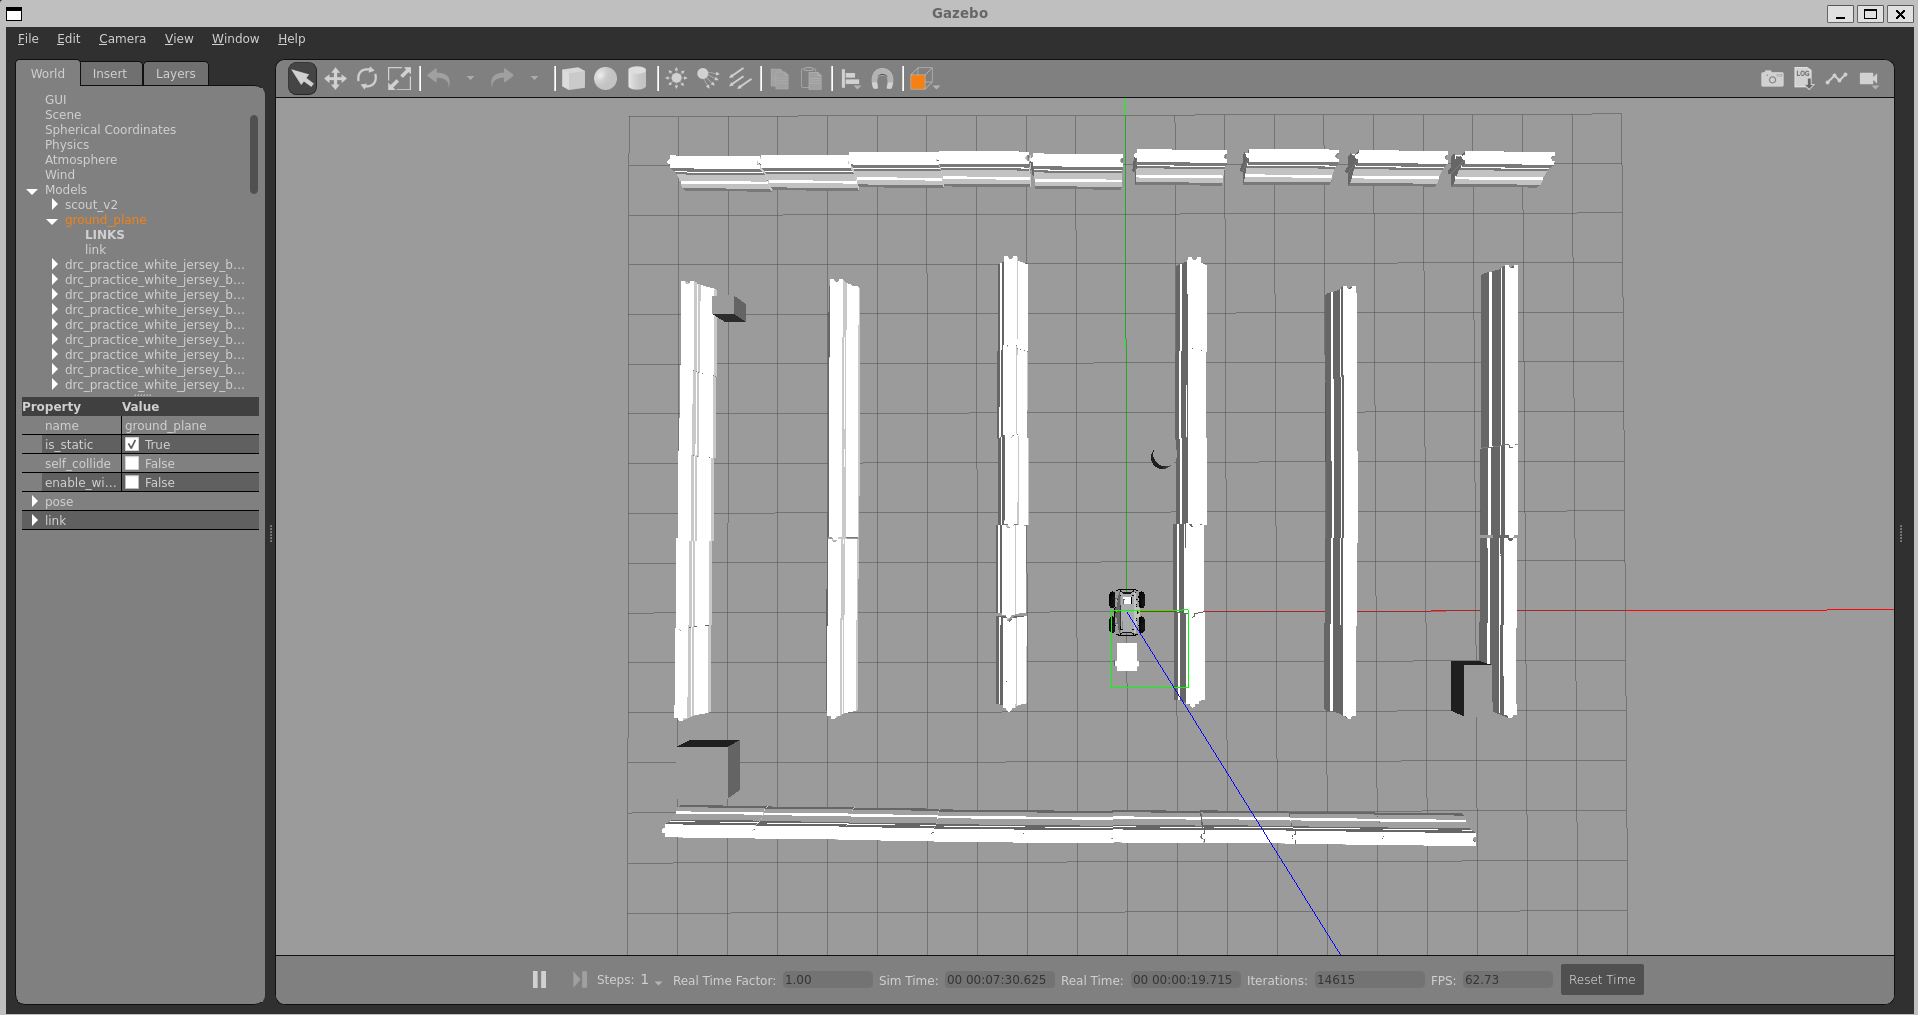
\includegraphics[width=0.9\textwidth]{gazeboworld.png}
    \caption{Gazebo world used for simulation.}
    \label{fig:gazebo_world}
\end{figure}


To visualize the robot in this environment as well as the different data that is deemed relevant a software called 
Rviz2 is used. This software allows the user to select the various \gls{ROS2} topics that are being published 
by the running nodes and visualize them in a 3D environment, which is very useful for debugging and testing purposes.
\begin{figure}[H]
    \centering
    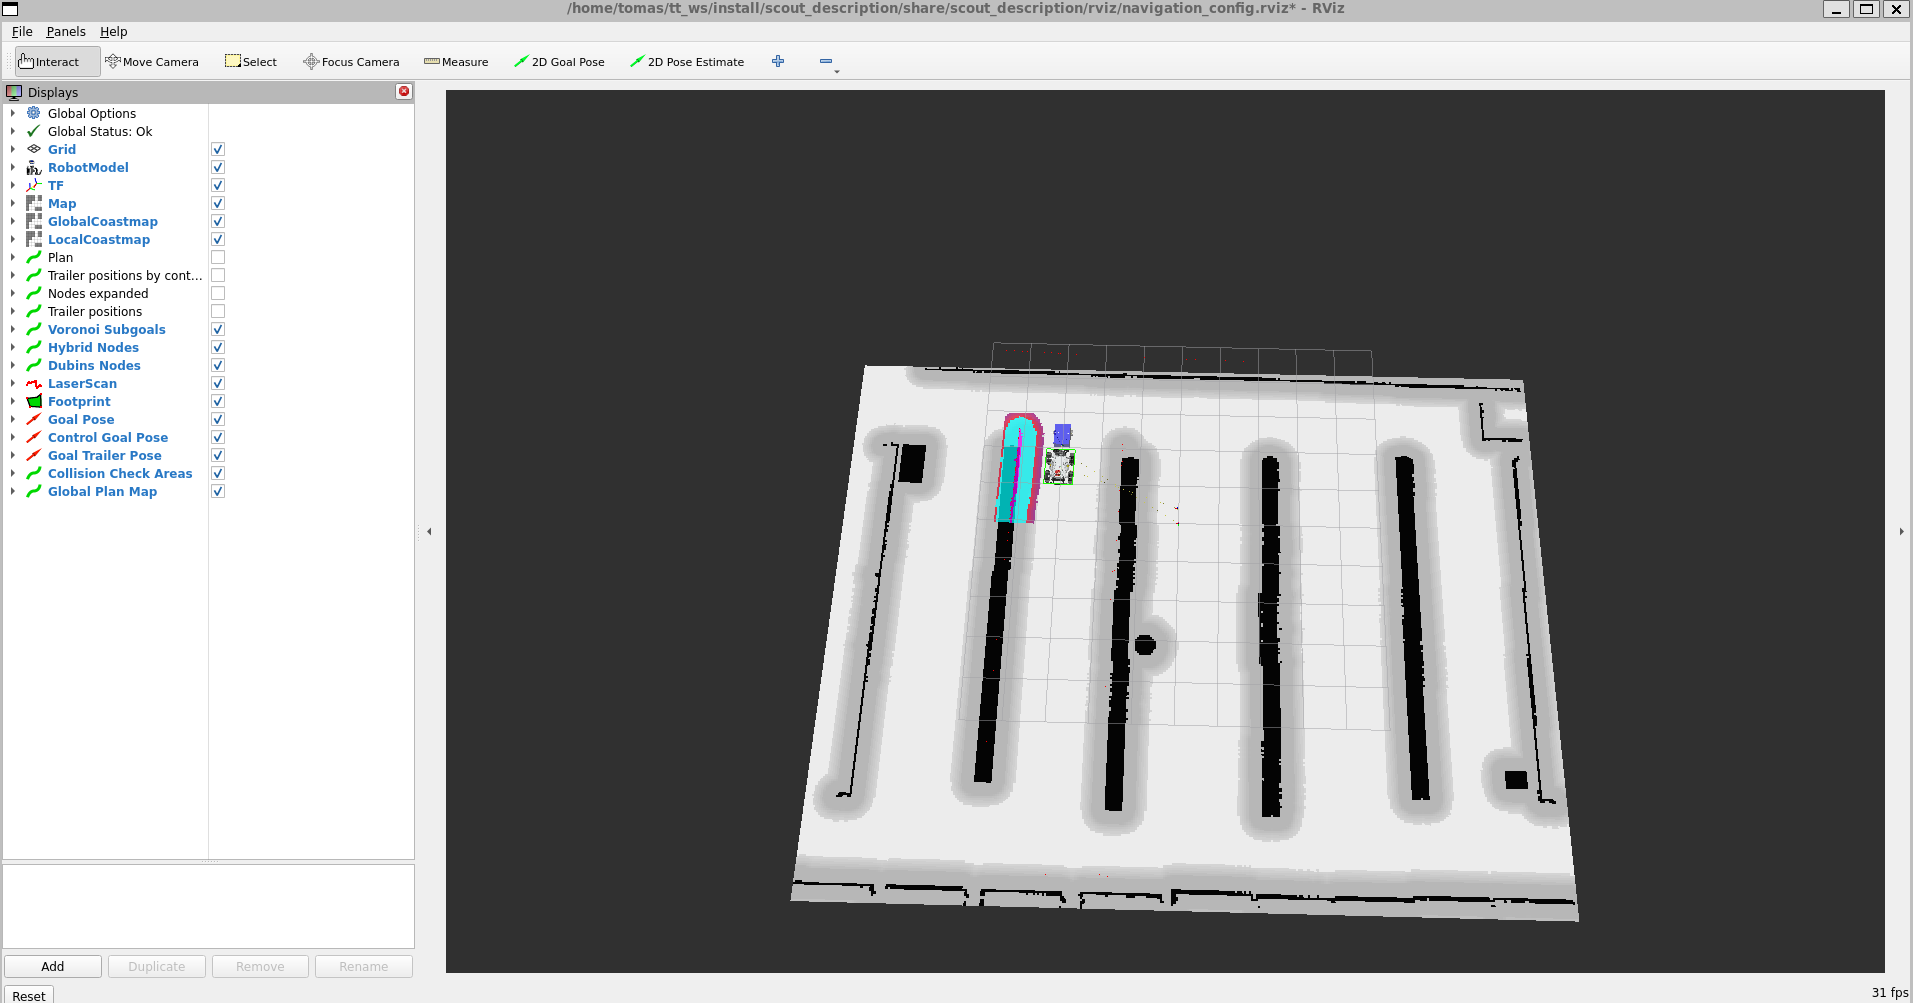
\includegraphics[width=0.9\textwidth]{Rviz2viz.png}
    \caption{Rviz2 visualization of the robot in the simulated environment. }
    \label{fig:rviz2_visualization}
\end{figure}

The figure \ref{fig:rviz2_visualization} shows, at the left, the different data provided by the developed system and, above it the 
navigation tools like estimatin the robot's initial position and goal generation. These last two tools can be used manually 
in Rviz2 or be published by a custom node if the user requires it.

In a first iteration, the prototype for the robot was also used in a real environment, a private room with a few obstacles 
and after mapping it could be represented by the following figure \ref{fig:basement}.
\begin{figure}[H]
    \centering
    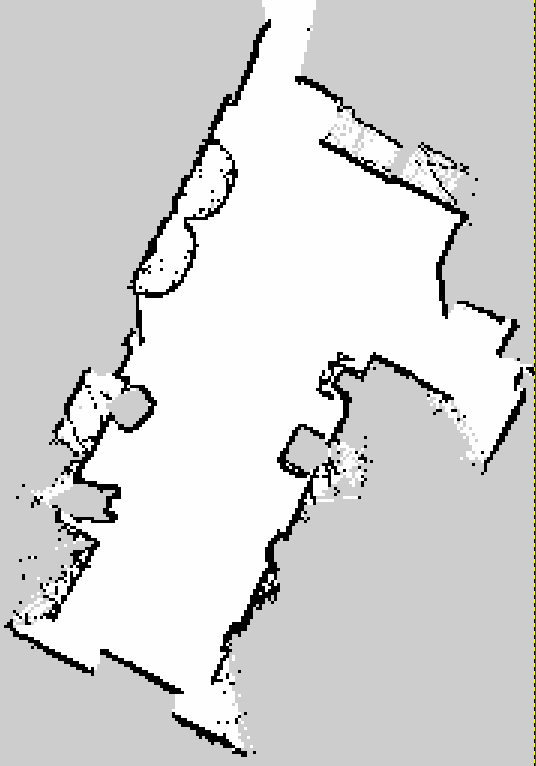
\includegraphics[width=0.95\textwidth]{basement.png}
    \caption{First environment used for testing the robot.}
    \label{fig:basement}
\end{figure}

\section{Planning algorithm}
\label{sec:planning_algorithm}

\paragraph{}As explained in the previous chapter \ref{sec:planner1}, 
the planner is devided into three main components, the Voronoi Graph, the Dubins Path and the Hybrid A* recovery algorithm.

\subsection{Voronoi Graph}
\label{subsec:voronoi_graph}

\paragraph{}The main function of the Voronoi Graph is to create a set of points in space that can be searched for a  
simple path to the goal using an A* search. Due to the nature of calculating a Voronoi Graph, it can be very computationally 
expensive, so the algorithm is ran offline, when the environment is mapped, and the resulting graph is saved to a 
file for the online planner to use. To create this graph, a Ros2 python node was created that executes a script with 
the previous behaviour.

The algorithm first works by creating black and white image containing the edges of the obstacles and grouping them 
into a single column of points.
\begin{figure}[H]
    \centering
    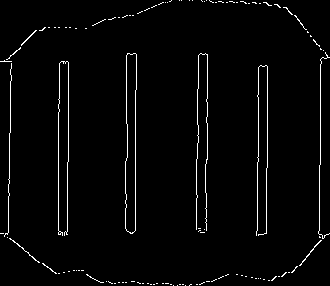
\includegraphics[width=0.9\textwidth]{edges_map_V20.png}
    \caption{Image with the obstacle edges.}
    \label{fig:voronoi_edges}
\end{figure}

\begin{figure}[H]
    \centering
    \includegraphics[width=0.9\textwidth]{voronoi_graph1.png}
    \caption{Voronoi Graph created for the environment in figure \ref{fig:gazebo_world}.}
    \label{fig:voronoi_graph1}
\end{figure}
